\documentclass{book}
\usepackage{graphicx}
\begin{document}

\title{FROM SINGULARITY TO DUALITY}
\author{Jure Šorn}
\maketitle

\tableofcontents

%=============================
%=============================
%CHAPTER 1
\chapter {From Object to Subject}
%13:12 15/3/04
Ok...

\section{So Hegel says about basic ordinary Knowing that...}

So I lost it. Not enough of a frame for me, but nonetheless, lets not get to pessimistic. If we take into account pursuit of Hegel's philosophy to resolve everything to its end, how come it's still able to posses structure instead of crumbling into itself. I think one must attribute this to the gaps; so this leads us to the foreground/background / chicken or the egg problem; what is more important/what was first: the philosophy/structure/wiesenshaft or the gaps/the incomprehensible.
As interesting and absolute as this problem seems it may be of little importance in itself unless we can render it to something a bit more 'earthly'; for instance: How does it relate to morals/primordial good/evil/... more specifically: can something already go wrong in this domain (rephrase)?
But to return to the notion of crumbling before. When does the philosophy/wiesenshaft begin to crumble into itself; and when it is standing, does it not all the time 'contain' this crumbling(or at least the notion) in itself. Isn't the concept of Now nothing but this crumbling into itself? So the question is how does it manage to remain, the-spite the crumbling which seems to be the essence of it? Well, it must be this unconectable gap between "now" and the last/next "now"; because although they are the same nows, and they stand one by the other, they just cannot be connected/merged/ or a little shifted, because of the notion of greater Now they impose. This notion of Now takes one of them and makes it a subject while other remains the object, and so although they remain the same, the multitude of them makes them different, and thus multiple; and we are back at the chicken and the egg problem. So we get this structure, but without the zero point, without the anchor. It's like if 2D fractals actually have somewhere between 1 and 2 dimensions and if Thought has only one dimension (that of cause and effect), then this structure lives somewhere between 0 and 1 dimension (effect effecting the cause). 
So with this established lets look at how it renders itself in physics. There we get instead of one, two ends of the thread. One micro and other macroscopic: neutrinos and galaxies.. So far, if we look at the material world as less pure then the spiritual (ideological), it makes some sense to have more ends. It also makes sense that the closer we get to the end the purer and at the same time more contradictory the forms get. But the question that poses itself here is: Is there the gap (this is different gap than one between nows) between the end and the forms or do the forms gradually morph into the void? And in the case of the physics will the knowledge (if it is obtainable at the first place) about one end imply the other; and since the is a 'lesser' world, will it tell us anything about the (non)existence of the primordial gap in the philosophical domain.
Of course the last question smells, but lets examine the different possible answers that Physics as such is capable of giving us: Discrete vs continuous basis, Singular vs multiple universes, Infinite vs finite universe, Lack of time vs lack of space at the big bang... So it gets clear pretty quickly that physical explanations of world at its ends automatically includes the spiritual (ideological).
But nonetheless (or because of it), the big question for/on both sides is the existence of the zero point and its relation to the void/non-existence. Is zero point same as void? But how can a point be a void at the same time? Isn't void the opposite of point, no matter from how far we look? If there is no zero point, then why does it seem like everything is pointing toward it?
To get a bit more metaphysical; Isn't the first and the only thing such entity as zero point can "do", to destroy itself by splitting into two parts, which of course cannot anymore be zero points, but one "positive" and other "negative" part of it. But since this jump looks like a necessity isn't it still in a way the zero point. I would say no, because it already incorporates something like a "decision": Which part becomes positive and which negative. This might seem like just a problem of naming things, but from where do we then get this notion of positive/negative. If it is from some later "event" down the line, how was than this primordial jump even possible.. But nonetheless maybe we are moving too fast here, specifically: Even though the primordial entity splits itself into two parts, and by definition this parts cannot be equal, because that would mean the entity multiplied itself, which would be impossible at this stage (because of lack of space for two of them:) and thus it can only split itself into two opposing entities, the "sum" of which is same as that of the entity itself; Nonetheless does the notion that they are opposing already imply that one of them specifically is positive? Maybe, but it certainly dozen't imply which, because they are also the same. Of course here we are already not only in domain of quarks, but also in part that of electrons. Although an electron cannot freely change into a proton; nonetheless the electrons themselves are indistinguishable among themselves - one is totally the same as the other (so it is meaningless to discuss for instance how any electrons that were once part of Buddha on average does a person contain in its body) - what keeps them in "order" is law of conservation. But again we are moving to fast here. 
We should examine the nature of the two Opposites some more. Precisely their being of the same matter, same ancestor, same cause, conceived at the same moment and still being different, maybe more accurate; being opposite. The question is from where does this concept of opposition stem. Is it already inherent in the Entity itself, or does it somehow emerge by itself from the impossibility of the Entity to "do" anything? Isn't thus the Opposition in opposition to the Entity(in itself/from itself)? The moment it emerges is itself in opposition to the Entity, but since this would mean the surplus, the original Entity must at the same time vanish, thus leaving the Opposition by itself -> what renders the two opposites, but also the opposition in the situation itself (namely parts being the same, but opposite at the same time), which is the real surplus we get from this split/jump. 
A quick and jumpy conclusion from this would be that, thus the wheels are set in motion from the start and the Jump is in it's nature an discrete event and thus the singularity unattainable by gradual deduction. And that the most primordial thing/idea that is accessible to us is that of opposition. And that it would actually enable us to grasp the singularity in it entirety if it wasn't for the opposition that it poses to itself by making the same at same time opposite. This surplus sets the wheel in motion, which makes it impossible to observe the singularity, also because we need the surplus at the first place to observe. -> This of course nicely parallels itself to nirvana experience, in which we have to lose more and more "stuff" until at the end we also have to let go of the observer/observer.

%=========
%15:50 15/3/04

\section{Good and Evil as primordial opposites..}

So the question that poses itself here is: What is the connection between good and evil and this two primordial opposites (and their surplus)?
In a way good and evil are the highest abstractions for the humans. We use them to substitute for us what is most important to us, although we always have trouble trying to label "stuff" with one or the other. We are also frequently questioning is it at all possible to bucket stuff this way; nonetheless the notion of Good and Evil is as present as ever. 
So to tackle it systematically, we have basically two possibilities: Are the two Opposites themselves good, because they themselves together alone are the Entity, and the surplus that stems from them evil? (Buddha) Or the other way around? (Judo/Christian - glorification of falling into)
Let's say that we identified the anchor of two different (opposite?) mortalities. How do we then get from this anchor to the other less general rules of morality (10 commandment, Buddhist basic morality,...), which are if we look at the world actually more general and present throughout cultures. Namely: Don't: kill, steal, be greedy, (angry, delusional), lie, slander.. One explanation would be that these rules are helping in maintaining larger societies and thus help in propagating themselves. So they are but the stage for the deepest morality which is one of the primordial ones, namely Buddhas: Don't conduct in sexual misconduct (excessive passion) vs Biblical Thou shalt not commit adultery and Thou shalt have no other gods which of course also serve the cause of propagating and same is with Buddha.
So by accepting this explanation we basically diminish those laws to the simple universal state laws, but at the same time we see between their lines their true meaning, namely taking sides in one of the primordial opposites. Two things of interest arise from here. First is if the majority of morality is strictly utilitarian in sens of trying to propagate itself, how would morality look in a world where opposite actions are necessary for a morality to propagate itself; namely: killing, stealing, lying.. of course inside of community itself. But this is definitely not as interesting problem as next one: 
----------
Let's take a little detour here and return to the Primordial Entity and its representation in Khmer/Hinduistic temples. It's beautifully represented in the biggest of them Angkor Wat, which represents the complete Hinduistic cosmos in small: Angkor Wat; All the elements of the temple point at the center and what actually is there is a deep hole, namely nothing. In the contrast to to Solomons temple, in center, the Inner House, there was the ark with ten commandments, which were given by God to Moses on Mount Sinai: in our terms the excess. Also worth of notion is the most predominant motive of the temples - The Churning of the Ocean of Milk - that is comes from hinduistic creation myth that talks about the game of thug of war between divinities and demons.
----------
But more interestingly, last distinction between essential/primordial part of morality and its utilitarian/reproductive gives us a chance to parallel (them) the two moralities to the two oppositions and their excess. This is getting a little confusing. Again: We have two opposing primordial moralities, and they form the excess which manifests itself in common moralities, which the two share. So if we look from judeo-Christian perspective to this structure, we favor falling in/sticking with them/embracing them, and from Buddhist perspective we try to "acquire dispassion for them". So from both perspectives, (common) moralities stand for a kind of a ladder, the only question is which direction is up, where should we climb? So are we to put them on the altar, embrace them fully again and again, let them shape our existence and follow where it leads us (thus basically abandoning their original context), or should we grow more and more dispassion for them, not abandoning them, but paving our path with them, thus giving less and less thought to them as we move forward with their help?   

Conclusion from above could be: Although the utilitarian moralities might seem like lesser ones comparing to the primordial, they are still moralities and thus in a way indivisible from each other. Although the judo and Buddha moralities are basically leading in opposite ways, it would be hard for one to label another as evil, since evil is supposed to be what lies outside moralities and both share commons which are indivisible from primordial part according to moralities. 
But if we assume both of them to be focused on their path, we can't but notice the very different perspective that is unfolding in front of them. To the Buddhist one, as it is moving along the road paved from basic moralities, the picture of primordial split is becoming ever clearer. And not until one can fully accept this split can one reach nirvana and thus basically abandon the road that let him achieve it. There is of course little need for god in this perspective.
The Judeo-Christian perspective, at the other hand, is facing endless road ahead, disappearing in haze. The possibilities for her are endless. Of course from this open position then stem endless controversies such as determinism/free will and god..  
%--------------------
%18:45 15/3/04
\section{A little appendix to the section}
BUDA: More we move this way, less lies outside morality -> we get enclosed by morality itself, but still, to reach singularity we have to cut off the excess, thus staying only with Buddha and Juda, which by this cut become the same. So the perspective before the cut would be very clear view of double opposite moralities.
JUDA: The other way that has no end (it is bodhisattvan by it's nature), it is surrounded by less and less morality, basically soaked in particularities, thus in a way penetrating deeper and deeper into god (void) (party getting out of hand)
Morality is in a way the last thing (frontier) that is of us, what is truly godly is outside morality, the void, the incomprehensible (the Random/ Mr Random). In other way, closing in to nirvana, god, Random, the incomprehensible is of less and less importance.
Thus the evil perceived as "stuff" outside moralities holds in the middle, but further up or down we go, we need a different approach to classification, (just) because of practicality.. In case of Buda side, Juda as evil would make sense, of course up until nirvana (still not answer to what can go wrong in nirvana domain) In case of Juda, almost fully emerged in god..., probably not not embracing more could be sign of evil (but that could also hold for Buda) But better question would be what is good? In a way notion disappears and we HAVE to trust god.
=====================
Is the third way the paganism - standing still on the leather? And what does Islam say (following rituals)?
=====================
%20:45 15/3/04
How to explain, by acquired means, the Tibetan position to the question of unnecessarity of morality to reach nirvana, that something can go terribly wrong in nirvana domain itself?
The way to start tackling the problem probably lies in the substitution of words by Zizek, from evil to 'terribly wrong'. It signifies the shift from our "earthly" moralities to some higher, but still maintaining the negative signifier. So instead of asking what could go wrong with nirvana domain, let's ask instead what does it mean for something to go wrong there, or rather what can even go wrong there, or even what can "go on" there? Isn't nirvana suppose to imply stasis?
First paradox here arises, that Zizek is trying to tackle a problem proposed by Tibetan tradition, within a scope of Theravada tradition. Particularly he is suggesting a problem in nirvana domain, but transplanted from a tradition with a different view of nirvana itself. Namely don't Tibetan Buddhist count the Bodhisattvas to be operating in nirvana domain itself. This domain seems different from Theravadean domain of nirvana which although after obtaining it you stay here and nothing changes is in a way purer shift than obtaining it and than returning. Theravadean nirvana thus doesn't leave you an option of getting back, precisely because you didn't went anywhere, where at the other hand one could imagine an Bodhisattva having an possibility of turning back and becoming "evil".
---------
correction:
At microscopic/macroscopic scale I forgot to mention of course big bang and big collapse, which are periodical cause and effect in Hindu universe. And also beautiful way one can represent them with the ways of the sky: N macro, S micro, E big bang, W big collapse.
=================================
Return to the Primordial Opposites
But of course the question arises: What comes next? Probably: consciousness, selfconsciousness, um, duh, religion, [absolute knowledge]?
So is there a middle road between Juda and Buda?
So according to Hegel if we go one level higher from the two religions we come to 'absolute knowledge'

=================================
Southeast Asia trip moments:
-When I should reply "We are all in this together.", to the "Worry, worry"
-You are a good man.
-(Buddha brought me to her.)
-(Centrality of the brothelo mall)
-(The reflex of the shoe and the money between breasts)
=================================

\begin{figure}[ht!]
\centering
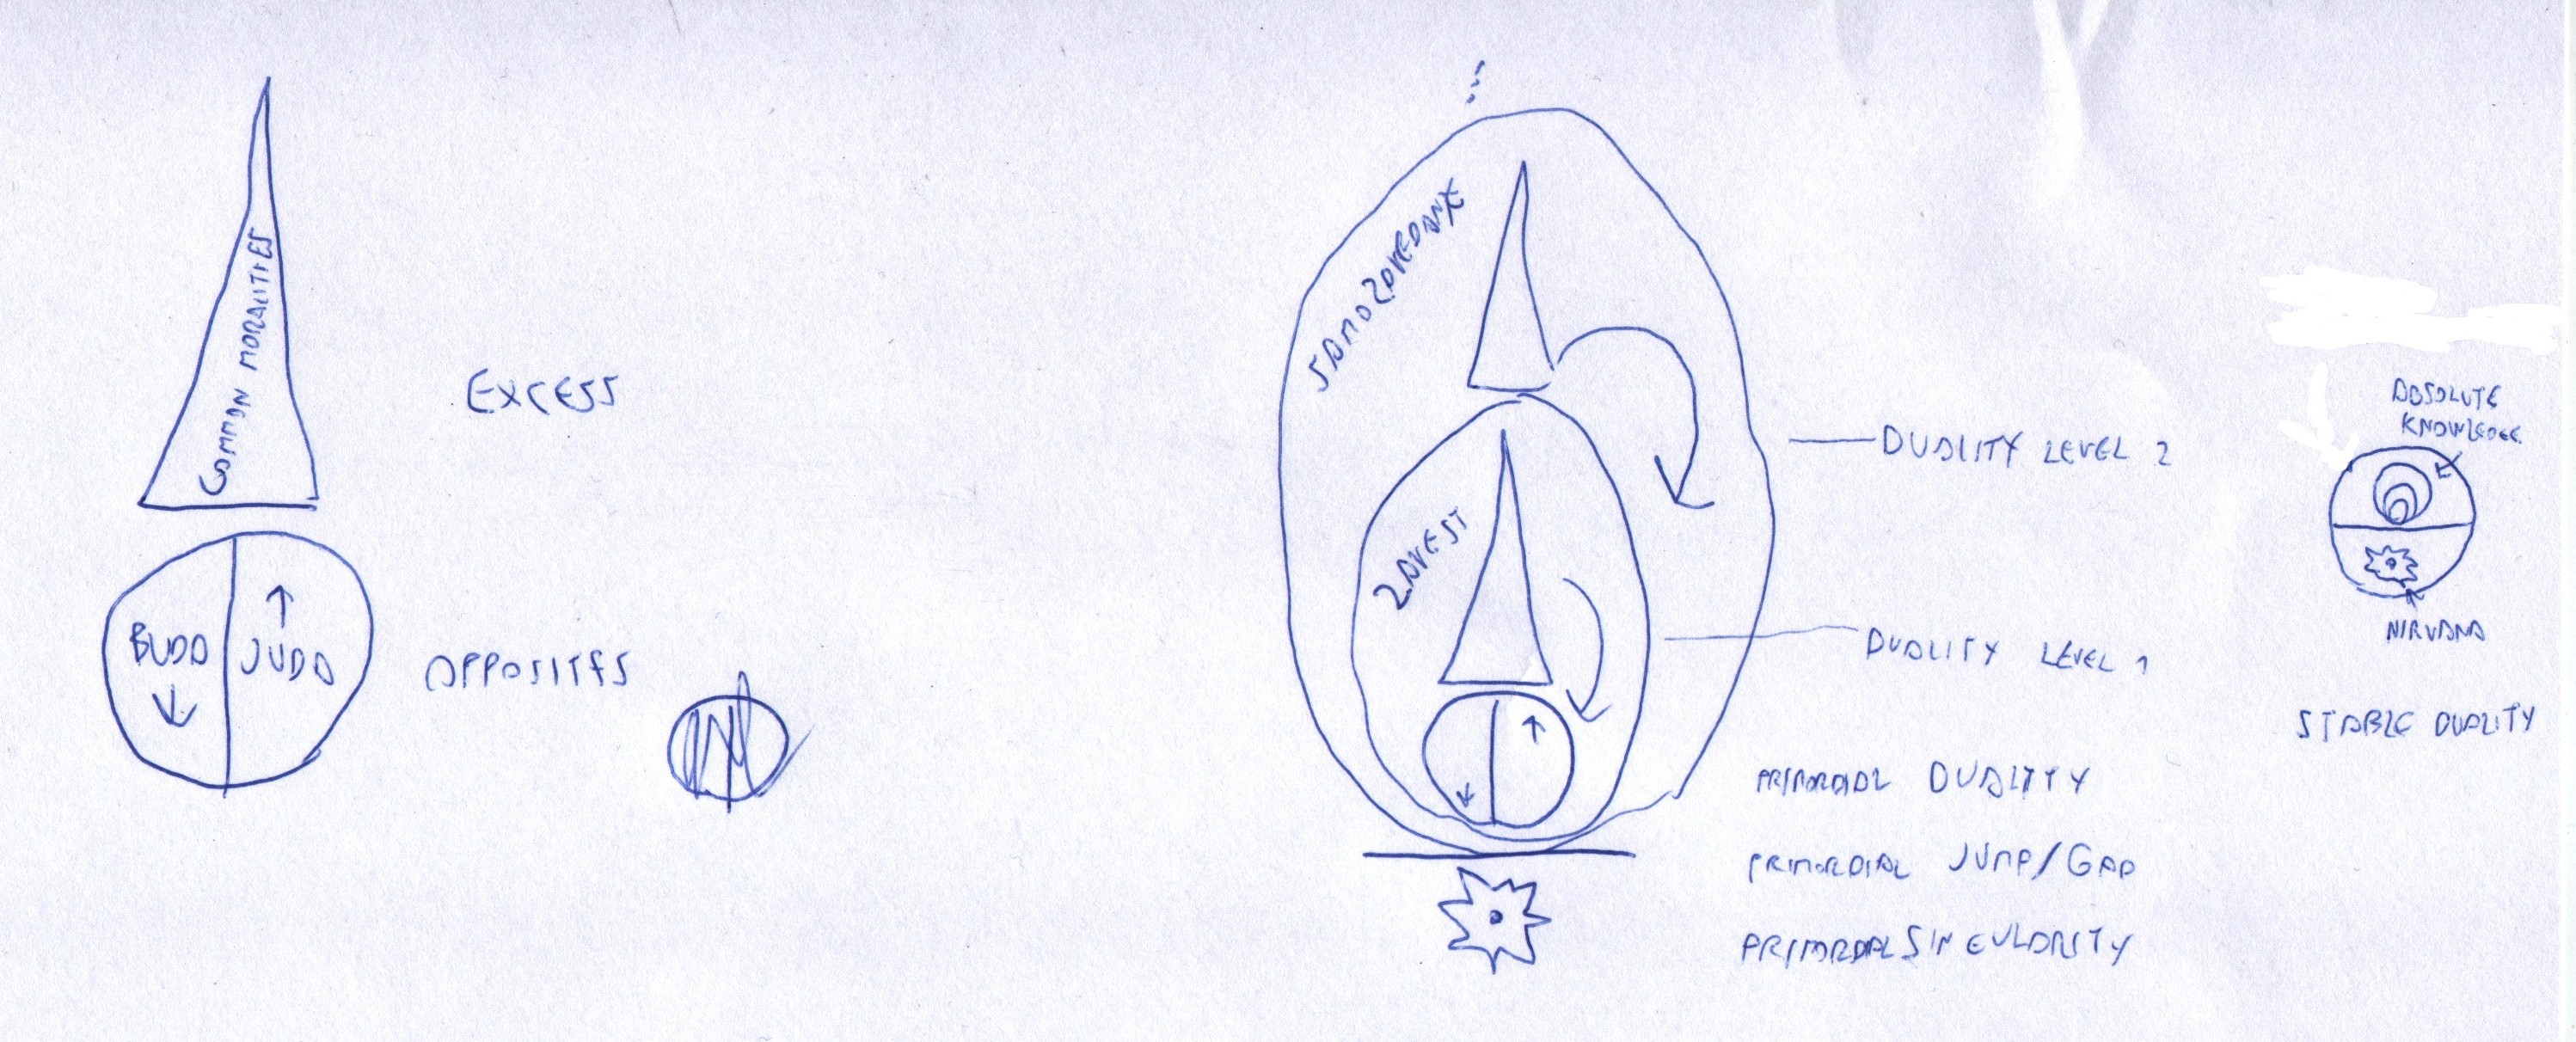
\includegraphics[width=120mm]{scan00.jpg}
%\caption{A simple caption}
\label{overflow}
\end{figure}

%14:30 16/03/14
From handwriting:
-The excess then becomes the opposite to opposites.
-TODO Further develop differences and commons between the commandments.
-TODO On which Hegelian level are we now (in this discussion)? Morals, religion, enlightened religion or absolute knowledge? 
-What could go wrong with nirvana domain itself:
1. UNDEVELOPED ((Only thing that could possibly go wrong is if there develops a duality in nirvana itself since it is only spiritual experience, of course is not physical, what means there is still a bit of excess, [but at this time its the excess of other, namely the excess of the spirit left behind - BLUFFING])) - is Zizek here leaning on Lacanian concepts?
2. Or is the problem the spirit that gets left behind? What happens to the spirit when it is abandoned? Does it become absolute knowledge? On the other hand, can only spirit because of its primordiality/spirituality obtain nirvana here and now, meaning obtaining it between the global nirvanas of big bang and big collapse)?
----------
Interesting correspondence of religious thoughts and scientific views of the universe:
1. Infinitely expanding universe - Juda
2. Statical universe - Paga(nism)
3. Collapsing universe - Buda
----------
For Zizek absolute knowledge (p48) is Lacanian passe: 
The final moment of the analytic process, "The experience of the lack of other" (p27). So in path of Juda this would be an Christian enlightenment - The death of god) So the moment god almost takes up completely it dies (the moment we or I attain absolute knowledge) And so through god everything is permitted (as long as one of course makes sure this path can be propagated (reproduced for others) -> as long as the framework, "empty" customs maintain -> catholic church / [Islam?]
So here seems that juda differs from buda: namely in the necessity of path -> where buda is free to abandon the "path" once it attains the enlightenment (at least in Teravada), to juda the conservation of the "path" after achieving enlightenment seems more important.
UNDEVELOPED But still as absolute knowledge is obtained through judo enlightenment, it can in a way let go of primordial singularity -> it in a way becomes a new singularity.. where as nirvana is obtained it can let go of all the dualities. - [Here it seams that as I am operating with this absolute concepts still too attached to the notion of self, as if one point is moving around the field, what can of course be useful analogy when operating around the middle, but as we are approaching extremes, the self is getting under attack.]
Absolute knowledge and nirvana as opposites(dualities).
In a way they don't contradict, they don't produce excess and thus they succeed in what the primordial duality "failed" at, namely creating stable duality (without excess)
But another reading could also be that only together they compose absolute knowledge?? But this would render juda and buda enlightenment the same, wouldn't it?
One can not attain the absolute absolute knowledge, one that would include absolute knowledge and nirvana together, precisely because they together form the stable duality, one without excess. And it is this lack of excess that "prohibits" the continuation of dialectical process, that would lead to next step, namely that of absolute absolute knowledge.
-----------------
%16:30 16/03/14
From Why Hegel is a Lacanian - drive against nirvana: Lacanian ethics
\begin{quotation}
Ethic and morality are to be sharply distinguished. Morality is concerned with the symmetry of my relations to other humans; its zero-level rule is 'do not do to me what you don't want me to do to you.' Ethics on the contrary, deals with my consistency with myself, my fidelity to my own desire.
\end{quotation}
---
From Hegel with Lacan: Differentiating absolute knowledge
Relation between knowledge and truth..
Absolute knowledge as abolition of the Other..
\begin{quotation}
One usually understands absolute knowledge as the fantasy of a full discourse, without fault or discord, the fantasy of an Identity inclusive of all divisions, whereas our reading, by way of contrast, sees in Absolute knowledge the exact opposite of this, the dimension of the reversing of achieved Identity where for finite consciousness there is only division rather the experience of distance, separation, where for finite consciousness there is only fusion and identity (between object a and the Other). Absolute knowledge, far from filling the lack sensed by 'finite consciousness' separated from the Absolute, transfers this lack int the Other itself. The twist introduced bu absolute knowledge thus concerns the very status of lack: the finite, alienated consciousness suffers from the loss of the object, while de-alienation consists of the realization that the loss of the object, while de-alienation consists of the realization that this object was lost from the beginning, and that any given object is simply an attempt to fill in the empty place of this loss.
.. To put it another way, the perspectival error consists in thinking that at the end of the dialectical process, the subject finally obtains that for which they are searching..
The passe as the final moment of the analytic process does not say that one has finally resolved the impasse, overcoming its obstacles - the passe can be reduced to the retroactive experience that the impasse is already its own 'resolution'. To put it another way, the passe is exactly the same thing as the impasse, just as the synthesis is exactly the same thing as the antithesis: what changes is only the 'perspective', the position of the subject.
\end{quotation}
----------
Sanja making Work, producing excess when working.
----------
The Tibetan rituals as empty framework.. because for common people they are the most effective method!
======================
%19:30 16/03/14
Hegel in phenomenology 780-784 (830-834 sl) Overcoming of good and evil
\begin{quotation}
780 So Hegel in resolved religion talks that in fact what is outside of religion is evil, or course until the religion itself doesn't realize that the evil in it self same as goodness, (and that evil being is seem as nature) .. (reconciliation of divine being with its other, specifically with a thought of it- evil. If this reconciliation is notionally expressed - .. - if evil is the same as goodness then evil is just not evil.., both are suspended moments, evil in general is self center being for self and goodness is what is simple and without the self.. their unity is at once evident.)
784 Christianity understood in this way leads to the idea that the coming of into existence of the gods individual selfconscusnes as a universal selfconscusness is the same as religious community. God the father and god the son are abstract moments until the emergence of the spiritual community .. community is the truth about those two moments... Divine being is a form akin to judging consciousness, acting consciousness (Christ), the mutual recognition between them is intuitively apprehended by religious consciousness as coming of the holy spirit..
787 Although there is a return out of picture thinking in principle in communal self-recognition, the community is not yet perfected this itself consciousness, and that picture-thinking steel burdens communal spirituality because it is jet to achieve pure thought. The community does not posses the consciousness of what it is. Substance has here succeeded in becoming absolute self-consciousness, but this remains at other for devotional consciousness. Christian consciousness is simply literally confused about its own fundamental commitments. It is confused not in sense of having contradictory beliefs, but because it expresses those beliefs in representational way, and the crock of this representational way is sometimes said,.. that the content of religion and philosophy are the same only expressed differently - this is essentially anti Hegelian form .. The notion of beyond becomes in Christianity simply the future - in some indefinite future at the day of judgment we will be resurrected, returned and finally united with god. .. The problem is a notion of beyond as the notion of the future. As long as word is waiting the dis-figuration, it is not taking the form of the spirit. So what makes the picture-thinking inadequate is its temporal schema, an idea of the discrete past present and future, and hence an idea of Christian time design in which good self-hood is an past event and an reconciliation happens in a distant future and the present is lost somewhere between manifestation and reconciliation. What makes representational thought representational is just understanding and therefore to get past representational and become conceptional what we require is a different way of thinking about time.
Discrete past, present and future.. we need different notion of time and history. .. Eruption of otherness for Hegel must be a wending of a kind which belong to the pain of dismemberment. A rending which no mere self-assertion can heal and hence requires the patience and the labor of a negative - a working through of a negative (traumatic history) History we read is history of trauma. In this was the phenomenology is about nothing else than the negative, for it is about nothing else but the various ways in which human beings have positive particular objects or forms of life as absolute and in each case has come to ruin. It it those ruins that slorvenge which have been our object. .. when i forgive you I already go beyond good and evil. The forgiveness is the denial that the morality is opponent. So there is something about forgiveness which is amoral. Rather then acting to evil we let it unfold.. [critique of forgiveness, forgiveness is forgetfulness, and i will not forgive / forgiveness has a standpoint of a annalist with respect to analyzed (Dostoevsky) -> literature] ..
\end{quotation}
%=============================
%=============================
%22:30 16/03/14
%CHAPTER 2 
\chapter {Nature of Being and the World}

1.How deep must we fall, before we can turn around and start climbing toward nirvana?
2.Do we attain the Object when we reach nirvana? Or rather do "we" become on Object when we reach nirvana?
3.And how come that the dialectic stops somewhere (at absolute knowledge)? And is there any property in primordial singularity (on it?) that is giving us the clue that the dialectic will have an end? (and does the number of levels have any significance? 5?)
%????????????????

Interrogating the real:
-Lacan - perspective of last judgment (which formulates the objective meaning to your acts)
-Saying "There us no big other" excludes this perspective (Derrida's infinite justice, forever postponed, always to come, nonetheless didn't make that cut)
-We need thi for truly autonomous ethic.

-Dialectical end: what was initially perceived as a problem is now seen as it's own solution..
-Zizeks open ended conception of dialectics!?!?
-How is Hegel's method not slimly the basis for new master signifier?
-Pvt Hegel's enlightened religion and its problem with time, where discerning big bang/collapse

A dot on time is line, a line in time is surface, a surface in time is volume, a volume in time is entity > we have 5 levels -> all we need to do now is get rid of time's temporal property, namely getting rid of past, present, future and we attain absolute knowledge.
Of course the dot is not a primordial singularity, even if in space of 0 dimensions, because it possesses its opposite > 0 dimension without a dot, namely the dimension itself. They are in a way primordial dualities, who's opposition produces excess, they resolve into the 1D space, since only way they can coexist is on a line (in time).
So we could ask here why not 5 dimensions? Does Hegel's dialectic have 5 levels because we have 5 fingers? Or because we live in 3 dimensions.
\begin{figure}[ht!]
\centering
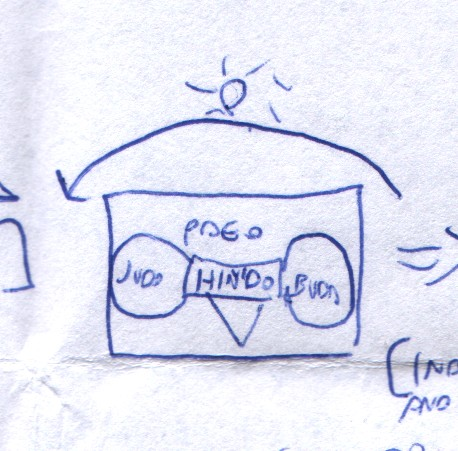
\includegraphics[width=90mm]{scan01.jpg}
%\caption{A simple caption}
\label{overflow}
\end{figure}
See how simple things as sunrise/set influence the basis of our belief! Namely buda in east, juda in west, and Hindu in middle (because India has both east and west shore, and paganism being to local to have any shore, and also Tibet having no shore) [is Hinduism the all encircling way?] Ko si na obali in gledas proti vzhodu, zahodu, en pogled je, da je bolk prirocno it v isto smer, drugi pa da seve civilizacije jasno vidijo kot center / najbolj razvito, ki je ze skozi tezila v to smer in prisla do obale [[neandertalci so sli v napacno smer:)]], pred nami je samo se veliki skok.

Katera lastnost singularnosti nam sporoca, da se bo dialektika koncala? 
To je verjetno znak prvega stavka: apak vseeno ne tako pesimisticno, kako da se hegklov system ne sesuje sam vase. Se pravi je to tisti hakeljc ki smo ga iskali, ne samo absolutno znanje, ki je sama realizacija, ampak opazka, da sploh lahko pridemo do brezoblicne singularnosti do realizacije. Zdi se nelogicno ampak ce prvo odvrzemo cas, ki ga moramo ze za absolutno vedenje, se nam lahko prikaze kot nuja? On the more philosophical level, although that we always expected to discover some "magic" at the end, when we do, it still seams impossible, although that it is in it's purest, nonrepresentational form the only way of magic to be, namely from faceless singularity to ending dialectic. Only other "magic-less" way would be for singularity to not explode. So in a way that excess of a jump renders itself in a finity of dialectic. (But we could probably also reverse it: So in a way that jump renders itself in a excess of finity of dialectic). To put it other way, the "magic" of a jump cancels itself with a "magic" of end of dialectic. Since we started with impossibility, isn't the only logical way that we end with one. 
So here we get a new duality, that between the jump and the end of dialectic. But they are not opposite!!! How do they correspond to the duality of singularity and dialectic (probably meant absolute knowledge). They are in a way endpoints, one of singularity and other of (primordial) duality / dialectic (i should be more precise here), but are also the endpoint of a stasis and of process/anti-stasis (only that the endpoint of process doesn't lead back to primordial singularity, bu to s stasis of a process/form) But the fact is they are not circular. the end of a process doesn't lead back to stasis (true/primordial singularity), nor thus it lead to new process; It just becomes the true (and only possible) opposite of it (primordial singularity). So loss is not perceived as such anymore. 

\begin{figure}[ht!]
\centering
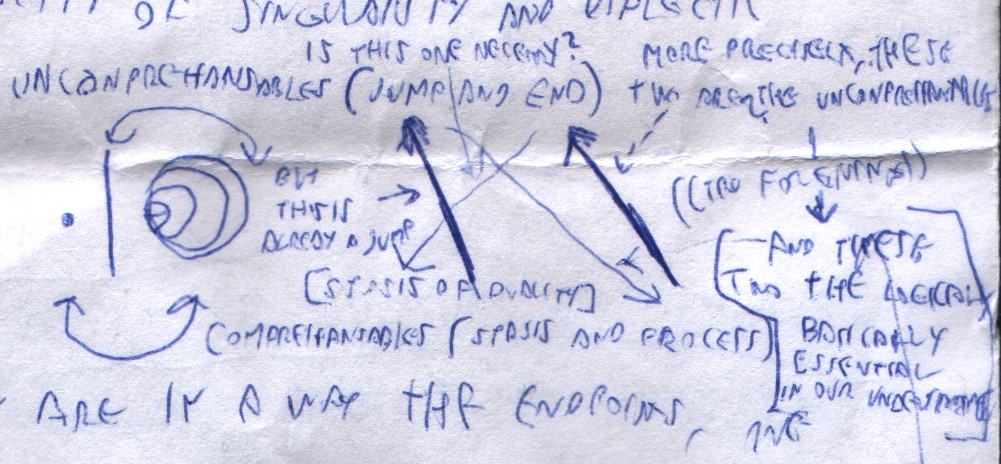
\includegraphics[width=90mm]{scan02.jpg}
%\caption{A simple caption}
\label{overflow}
\end{figure}

How deep must we fall, so we can start climbing back toward nirvana?
Simple answer: Deep enough that Buddhism can form. So probably enlightened religion? So all the way to the last step before absolute knowledge (?) So the entry point to enlightenment for both juda and buda is at the same end edge of progress, namely the enlightened religion, only that one offers a step out ant another a slide back into the beginning. (refine)

To take it afresh, why is the end of dialectical process essential?
Of course the singularity and duality/absolute knowledge do not posses in themselves the opposite (really?). For absolute knowledge, the singularity is list and for singularity the absolute knowledge is unattainable. They are separated by the jump. So from this distant perspective jump loses it's directionality and becomes just a barrier. (we just happen to find ourselves on this side) So is the question how did we come here (find ourselves on this side)? No! The question that makes sense to us should be: Should we embrace it or escape it (distance ourselves from it) (the side). So we can look at the two paths (given to individual) as the only true alternatives, that in a way can't produce an synthesis, and thus as only true ethics. But of course one can choose to follow one half of his life one and the other the second. But not I think, if one follows juda, he in a way never stops; he embraces the embracement and so on.. The moment one stops, and turns around, he becomes unethical.
And when one reaches nirvana, well he stays in this world, and can teach others and offer them support,but what are his ethics after nirvana?
----------
Kindergarten between German and American embassy.
---
Since we accept the impossibility of a jump (went that way), we are forced to accept (we must) the impossibility if a end of dialectic.
----------
Both ways of course require us of letting go of the pictorial representation and of notion of present/past/future, thus both ways must let go of a ethics (morals) that require final judgment, or even the notion of it (even if unattainable). One ethics that can do without it. Well, doesn't he who becomes just the observer of a samsara, doesn't he loose ethics as such. Don't ethics only exist in a domain of absolute knowledge? But when one obtains juda enlightenment, does he step out? No, he is out of enlightened religion, but still inside absolute knowledge.
So is this level attainable for someone who is trying to reach nirvana?
In a way ethics is all that remains in judo enlightenment (ethics of ethics) (and thus they consume morals) and totally disappear in buda enlightenment. (In both cases morals are probably the first victim) [So only ethics of the commandments remain at this point, but this is probably one step before the enlightenment] > probably the ethics of juda enlightenment > nirvana as abandonment of ethics > is this even bearable for human/spirit > 
Does one abandon spirit too (along with ethics)?

So if we arrived to the end in a spiritual domain, will this render itself as achieving the end in hard sciences too, namely physics? Will we finally succeed in getting rid of time? And will it not lead us to the same end as philosophy, namely the finding of the magic, but that magic being the only possible one, so in a way a bit of disappointment for us. Will it not lead us to the duh.. moment. (Like what did you expect? Something to end, and not be magical at the same time?) But lets dwell a little more here. How specifically would that be stated in physics?
So the magic of a center/big bang requires a magic of its edge/end/finity. The universe can not be infinite, or at least have infinite mass/energy. [where do infinite universes fit?] As effect without a cause the impossibility of a jump(big bang) realizes the impossibility of a finite mass/energy and the impossibility of a finite mass/energy requires an impossibility of a jump/big bang. (as what is then on the other side of an edge of universe?)
Buda/juda?
And since big bang and big collapse are from a distant perspective, without a temporal dimension, basically the different manifestations of the same thing, namely the primordial jump/gap, we are only left with two concepts: gap and here (universe) and thus singularity is forever lost for us, but the loss enabled our existence, so we get at least that :)
So the wrong way of predicting what that would manifest itself in physics is that the system (of equations) is the singularity we were looking for, although we will never find the missing part of equation, because it doesn't exist, so in a way we will be forced to put in a most imminent spot of a final equation one blank variable (lambda, one that can be substituted with any equation, thus also with itself.), and thus we will conclude the circle; Finish and connect the system.
(That would probably stand from Bach/godels perspective, but not from Hegel's. But even from his/theirs perspective, aren't fractals bounded on one side; they have surface (at least some), are not infinitely big; they only have infinite edge.. Bach/godels as Hegel for the Anglo-Saxons.. Do they think the path is infinite?) But this would probably mean the endless recursion and thus endless dialectic. More Hegelian would be stance, that we will find the last equation, but that alone will imply, that something must have been left out. We still won't be able to explain big bang/collapse, but this exactly will require big bang/collapse to have happened, this will be it's explanation.
So to put it in a way less dramatically: One can't get a big bang/collapse withouts a closed system of equations, and one can not get closed system of equations without a big bang/collapse. 
[question that still stands is how come did this equations and system become so balanced]
Both are irregularities, that "cancel" each other out, or better constitute the underlying composure that both sides need [articulate], although they are entirely separated.
So even singularity in a most primordial sense needs (or already possesses in its self) our universe, although it may seem self-sufficient. 
[So the question that remains is: Why do we then perceive singularity as self-sufficient?] So to put it simply, we are to accept the impossibility of true/stable primordial singularity. [Are we? What about nirvana?] Is not nirvana as such, obtaining this or at least some singularity?
Science:
So will not equation at the end connect (make sense), but their exclusion of a big bang/collapse will not make sense, so we will get that it was lost from beginning [big if]
Magic:
At the end when we find it, isn't that act of finding it exactly the magic itself, and thus the only imaginable way of finding one. More precisely, the magic that we find is not the object (singularity) itself, but the fact that we are able to accept, that it was lost from the beginning. The possibility of our search ending without finding it is what is magical (or the actual magic) and incomprehensible.
So in a way that two magics are then in a way true duality, one in which singularity tried to split itself into, but failed. True (stable) dualities in sense that they are opposite, but not opposing, the true two faces of a coin, that do not generate excess. So in some way they are the two bounds of our world. (In physics finite time and finite space, or better that of micro and macro) So on one side magic of the gap bounds us from the singularity/object and at the other the magic of attainability of absolute knowledge bounds us from the infinite other, from the void. (So in a more physical language big bang preventing matter to get infinitely small (disappearing) and a system of equations/laws, preventing matter to be infinite) If this bound would be missing and the equations would not be closable, it would mean our universe would be a fractal..
So with an act of splitting, singularity succeeds in bounding itself (buying herself structure, for the price of substance) Although she was self sufficient, she was missing structure, and although we have structure, we are missing substance. So in a way she exchanged her being/essence/center for structure, she turned herself inside out, got rid of a substance. (Like Johnson sells its soul to the devil for the success; changes his substance for structure)
Religion not seeing itself as the other "magical" boundary. 
\begin{figure}[ht!]
\centering
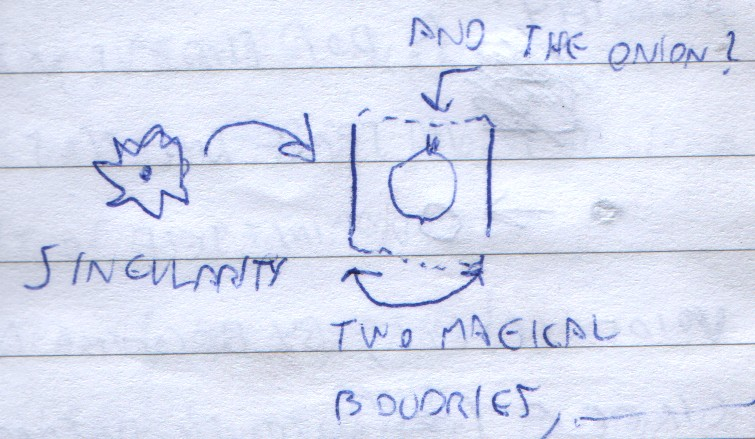
\includegraphics[width=90mm]{scan03.jpg}
%\caption{A simple caption}
\label{overflow}
\end{figure}
Two magical boundaries (that are of the same), which give rise to structure without substance; the onion.
So to put it very simplistically, we are at the problem of figure ground, and singularity changes from a dot to enclosing space, where structure is possible, but even more simplistically and maybe accurately: a dot that is not in space and thus in-itself, 
\begin{figure}[ht!]
\centering
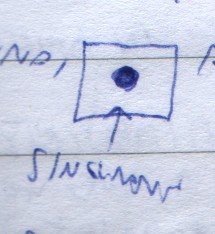
\includegraphics[width=90mm]{scan04.jpg}
%\caption{A simple caption}
\label{overflow}
\end{figure}
voids itself, by becoming a circle (shape without surface), and thus with loosing its surface enables a structure to emerge in-itself [isn't this pictorial thinking?]. But even more mathematically correct, a dot (not a sphere) expands itself into a circle in one step (what is morphologically impossible; It should first become a line, which then connects its ends - that way former analogy is better)
\begin{figure}[ht!]
\centering
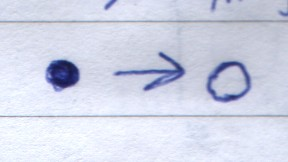
\includegraphics[width=90mm]{scan05.jpg}
%\caption{A simple caption}
\label{overflow}
\end{figure}

[cocaine vs LSD]
magic:
So the solution that would not require a magic would be one of recursion, namely that electrons would be just a little planets, and so on (universe of infinite detail and size), and since this is not true, we absolutely need little "magic". So this "magic" is precisely the magic of possibility of primordial jump and that of possibility of absolute knowledge, which are two sides of a coin. So through the magic of absolute knowledge/end of dialectic, we realize the magic of primordial jump/gap, that it really happened. So singularity exchanged it's infinity that it possessed, for structure. So it seized to be total, for the ability to be creative. [Here we look at it trough form of a story; of course more singular/absolute way of looking at it would be that, singularity already possesses in it's essence structure] [but it also probably bounds itself with time; but this seams a little high price to pay for a jump - it would be ok if it would endlessly expand and contract, so to give some dynamic structure to it]
Which religions/believes do not have the end of time? That would explain an non-urgency to go either way on the leather.
So the magic of the jump implies, that there exists the smallest "object" "under" which there is nothing
So the circularity of a universe (time) seems the only logical system in which we don't "bound" time, but still maintain its temporal/action giving component.
But this of course rises the question of what would happen the moment one universe isn't contactable. This would of course stop the cycle. So a better solution would be a infinity of universes, all going of at the same time.
And out of this course comes big question: Can we cheat it? Can we influence in any way the next cycle? [a bit too sifi, but also maybe not relevant?] Are we ourselves (our cycle) a product of this kind of cheating? But more importantly, what would this "cheating"/gluing together/transcending of the cycles mean for the time and universe itself?
And if there can not be any influence, does this mean that all the cycles are exactly the same (that would be kind of disappointing :( Of course here rises the question of determinism: Are all cycles the same or do they take up all possible (stable) forms? [The later way gives rise to interesting parallel to quantum physics: So in a way we have free will, but looking at the big picture, our choice ends up just as a part of a graph of normal distribution. So in a way it is known beforehand how regularly your act will occur, only it was not known that it will happen precisely in this cycle. Or better: we will choose one way and thus have free will as long as there exists an observer, otherwise our actions will spread nicely trough specter - we will choose both ways simultaneously (if we reduce choice to two paths). The question that of course remains is are we enough of a observer to count:) ]
[[why does so frequently when one tries to blacken other religion and believe his; he sounds like someone is making a joke? Trolling for the fun of trolling. Nature of trolling; Opposing for the sake (fun) of opposing. Troll as agent without substance, without its own position - position shifts depending on a debate, and is always anti.]]
%=====================
%=====================
%19.03.14
Space:
So the space (void, other) itself can be infinite, but it doesn't mater to us as long as mass/energy/structure [absolute knowledge] is. 



From interrogating the real - why is Hegel Lacanian:
\begin{quotation}
In the domain of knowledge, we encounter this logic of separation when, all of a sudden, we see that what we thought was the limitation of out knowledge about the thing is in fact an inherent limitation of the thin itself. Recall Adorno's analysis of the antagonistic character of the notion of society. In the social sciences, the notion of society oscillates between two extremes. Either we conceive of it in terms of Anglo-Saxon individualistic-nominal-ism, as a composite of interacting individuals as the only really existing agents, or else we adopt a more Continental perspective, exemplified by the work of Emile Durkheim, and conceive of society as an organic Whole, a totality that pre-exists individuals. The antagonism is here irreducible, and we seem to be dealing with a true Kantian antinomy (the existence of two mutually exclusive, contradictory even, claims that are both equally justified) which cannot be resolved through any higher dialectical synthesis: society as such cannot but appear as a Thing-in-itself, forever out of grasp of our cognitive capacities. However, as a different approach, one should merely observe the way that this radical antinomy, which seems to preclude our access to the Thing, is already at work in the Thing itself: the fundamental feature of today's society is the irreconcilable antagonism between social totality and individuals. What first appeared as the sign of our inability to understand what society really is turns out to be the fundamental feature of social reality itself. That is to say, initially, we were 'alienated', our limited knowledge prevented us from achieving a notion of society; then, in a properly dialectical reversal, this limitation proved to indicate the antagonism of society as such.
\end{quotation}
\begin{quotation}
Buddhist Ethics: In the Gnostic mode, for Buddhism, ethics is ultimately a question of knowledge and ignorance: our craving (desire) - our attachment to terrestrial goods - is conditioned by our ignorance, so that deliverance comes from proper knowing. What Christian love means is that, on the contrary, there is a decision not grounded in (true or false) knowledge- Christianity thus breaks with the entire tradition of the primacy of knowledge that spans from Buddhism through gnosticism to Spinoza.
\end{quotation}
\begin{quotation}
Buddhism/Psychoanalysis/Hegel: In what , then, does the gap that forever separates psychoanalysis from Buddhism consists? In order to answer this question, e should confront the basic enigma of Buddhism, its blind spot: how did the fall into samsara, the Wheel of Life, occur? This question is, of course, the exact opposite of the standard Buddhist concern: how can we break out of the Wheel of Life and attain nirvana? (This shift is homologous to Hegel's reversal of the classic metaphysical question, how can we penetrate through false appearances to their underlying essential reality? For Hegel, the question is, on the contrary, how has appearance emerged out of reality?) The nature and origin of the impetus by means of which desire, its deception, emerged from the Void, is the great unknown at the heart of the Buddhist edifice: it points toward an act that 'brakes the symmetry' within nirvana itself and thus makes something appear out of nothing (another analogy with quantum physics, with its notion of braking the symmetry). The Freudian answer is drive: what Freud calls Trieb is not, as it may appear, the Buddhist Wheel of Life, the craving that enslaves us to the world of illusions. Drive, on the contrary, goes on even when the subject has 'traversed the fantasy' and broken out of the illusory craving for the (lost) object of desire.
Death drive/nirvana principle: This is what Lacan aims at when he emphasizes the difference between the Freudian death dive and the so-called 'nirvana principle', according to which every life system tends toward equilibrium, the lowest level of energy, and ultimately toward death. 'Nothingness" (the void, being deprive of all substance) and the lowest level of energy paradoxically no longer coincide; it is 'cheaper' (it cost the system less energy) to persist in 'something' than to dwell in nothing', at the lowest level of tension, or in the void, the dissolution of all order. It is this distance that sustains the death drive (i.e. drive as such, since as Lacan puts it, 'every drive is virtual a death drive'): far from being the same tension, the longing for return to original nothingness), death drive is the tension that persists and insists beyond and against the nirvana principle (the striving toward the  dissolution of all tension, the longing for return to original nothingness), death drive is the tension that persists and insists beyond and against the nirvana principle. In other words, far from being opposed to the pleasure principle, the nirvana principle is its highest and most radical expression. In this precise sense, death drive stand for its exact opposite, for the dimension of the 'un-dead', of a spectral life that insists beyond (biological) death.
\end{quotation}
\begin{quotation}
Islam: Thus us why psychoanalysis is firmly entrenched in the Western Judeo-Christian tradition, as opposed, not only to Oriental spirituality, but also the Islam - one of the religions of the Book, which , like Oriental spirituality, endorses the notion of the ultimate vanity, illusory nature, of every object of desire.
\end{quotation}
\begin{quotation}
Lacan: Maintaining the gap that forever separates every empirical ('pathological') object of desire from its 'impossible' object-cause whose place must remain empty? Is not what Lacan calls 'symbolic castration' this very gap which renders every emorocal object unsatisfactory?
\end{quotation}
\begin{quotation}
Lacan: Absolute Knowledge is not accomplished symbolization.
\end{quotation}
\begin{quotation}
Crusades: In order for us to experience the spiritual truth of Christianity one must first occupy the tomb and then experience its emptiness - it is only through this disappointment, through this failure-in-triumph, that one gains insight into how, in order to -live in Christ; one does not have to go far away and occupy empty tombs, since Christ is already here whenever there is love between his followers.
\end{quotation}

%=====================

One could also draw a parallel between a spiritual and material world as one representing primordial singularity and other the other side. But that would then mean: 
\begin{figure}[ht!]
\centering
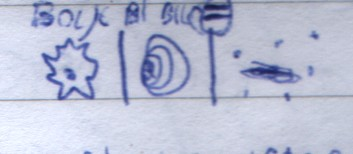
\includegraphics[width=90mm]{scan10.jpg}
%\caption{A simple caption}
\label{overflow}
\end{figure}
a twofold explosion (weird). According to this ideas exist before big bang, but the need for it seizes!!! Or maybe just that for us the big other is our universe. -> Better not to mix "stuff"/dimensions for now.

Drive: So you don't see "drive" in a universe. Maybe it was here only in the beginning, taking form of a inflation.


%===============================================================
%===============================================================
%CHAPTER 3
\chapter{Juda vs Buda}

Does Jump/end duality correlate to singularity/absolute knowledge duality? What is their relation? Probably they are figure ground. [Develop it further!]jump-end = big bang/collapse-micro/macro barrier.
1. Get rid of time: bang = collapse
2. So we get three: bang/collapse, micro, macro
3. Other: space + time
4. Absolute knowledge: final mass/energy + finite cycle

SIMPLISTIC:
So since we live in a physical world, which is lesser than the spiritual, we have two others, and thus four barriers, two for every other.
PROBLEMATIC:
So bang/collapse are of the same, but micro/macro are not. (We could probably still have finite mass with infinite detail, and infinite mass without infinite detail.) But with time: time without end and time without beginning equal in length to time without both. They are all infinite.
\begin{figure}[ht!]
\centering
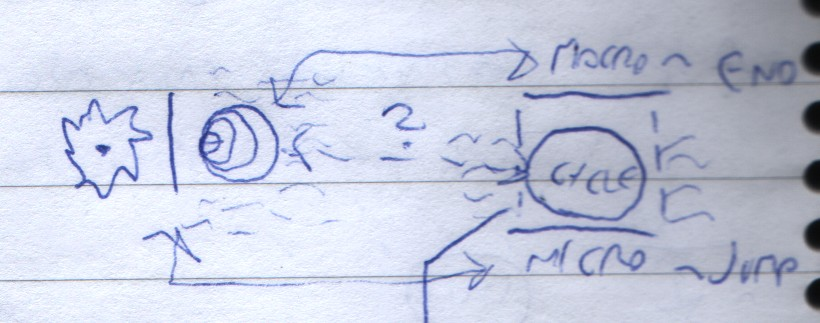
\includegraphics[width=90mm]{scan07.jpg}
%\caption{A simple caption}
\label{overflow}
\end{figure}
\begin{figure}[ht!]
\centering
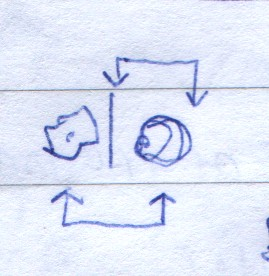
\includegraphics[width=90mm]{scan08.jpg}
%\caption{A simple caption}
\label{overflow}
\end{figure}
So how does this two correspond? (singularity and absolute knowledge vs jump and end)

How did we get time? [It seems mandatory for thing to happen, but still] We don't need it in spiritual world. It seams rational that we need it, but from where did this "extra" dimension came? [From where did any dimension come? From dialectic?] 
----
Zizek talks about symmetry within nirvana... So nirvana is not obtaining primordial singularity of course, but primordial duality!!! Duh. So a state without a consciousness. (nirvana = object a)
----
-Budas and Judas image of each other, and a possibility of a middle ground (buda is already middle way).
-Almodovar: All about my mother.
?????????????????????????????
					buda		juda
Intoxication:		no			yes
Falling in love:	no			yes
Spreading the word: no			yes
God:				indifferent	is dead
Salvation here:		yes			no

\section{All about my mother}
So lets take Almodovars movie All about my mother as an example of juda advocate. In the movie we get one possible representation of a guy who reached nirvana from the juda perspective, namely Rosas father. He has an advanced Alzheimer's disease, he cant recognize Rosa anymore and his only question to a strangers are "What is your age" and "What is your height". So the scene when they meet, is when the two worlds meet. Rosa as true juda, nun who is about to give birth (and also die at the same time) and her father. But the magic in this scene is that the encounter works for both. He asks her about her age and height, she answers, and they are both satisfied. But there are two prerequisites for this scene to work. First is fathers dog, whom Rosa calls to the taxi and father then fallows and Manuela as a witness to this (big other?) Of course here is also a taxi driver, but he like all other true men in a movie are absolute non-agents/non-actors (don't have impact on the story) and thus can't count as an observer. So with the dogs ability to recognize and share his excitement with Rosa versus fathers inability we get the ultimate insult to the buda. Her father stand here for the ultimate non-agent, less than unconscious animal. 
So some kind of conclusion here would be that if you are unable to fall, you are also unable to act. But there are two ways of falling. One manifest itself in the theater/spectacle (Barcelona) and other in stable (motherly) love(Madrid). And dividing her live between this two (passage between in movie is represented by a tunnel) is what at the end brings happiness to Manuella. So to be more precise, one way is falling into falling, attaching one self to attachment, kind of a spinning snow ball, embracing the world (here we are probably very close to buda), and the other is an attachment to an object (sun). What we don't get in buda, is this back and forth movement. We only have before and after nirvana. But more importantly we have this ideal of a middle way. (What is also interesting is geographic position of Barcelona, as one of a few European cities facing east. There also one could mention Pattaya as a sort of eastern Asia's Barcelona; one of a few cities there facing west)
So it could be said that for Almodovar the main actors have obtained a kind of nirvana. Although they are still aching and loving, this doesn't stop them. They live in this samsara, where identities are fluid, nothing is certain and are nonetheless capable of keeping distance. (nice cul de sac scene) But what is really nice it's the effect that it has on a viewer, namely the simultaneous crying/laughter (tragicomedy par excellence). More precisely, we sympathize with actors (agents), but also acquire a distance from density of events. More precisely: The density disables us to emotionally process everything, and thus it pushes us to a far perspective, from where we are able to see a farce of a big picture.
[[(Almodovar: You are what you perform)]]
So one conclusion from film would be that buda is about always taking the middle way, and juda about oscillating between attachment and perpetual falling with a stoic/nirvana attitude.

So is Almodovar buda after all? There is one aspect of a movie left, namely the moral of a story, who loses at the end. Loser is Nina. An only true addict (junkie) and in a way only "normal" woman in a film. (She gets married to a real man (non-actor), leaves the theater/Barcelona and gives birth to a ugly baby, thus she gets deprived of a stable/motherly love.) So he stands for reminder that there also exists the wrong kind of falling/attaching. Her attitude toward her own addiction is probably the strongest signifier: "I trade it for a bit of peace". In other words, I do it just to make everything a little easier (like a thing on a side) (Also a remark from Agrado: That fix didn't agree with you). So the her problem is not embracing enough/ trying to "dampen" a little everything. (Bad karma?)

So back to is Almodovar advocating buda, or maybe some middle way between buda (middle way) and juda?  

---------------------------
From Buddhist websites:
\begin{quotation}
Loving kindness, compassion, appreciative joy and a particular form of equanimity are the four kind of love taught and encouraged in classic Buddhist teachings. None of these are uniquely Buddhist; they are four qualities of heart that reside within everyone, at least as potentials. Teachings about the for forms of love existed in India prior to the Buddha, they were elements common to the Indian spiritual world which he included within his system of practice. While Buddhism cannot exist without love, it may be helpful to realize that love can exist happily apart from Buddhism. Learning the ways of these four loves does not require one to become a Buddhist. It only requires a willingness to develop innate capacities.
Love does not need to be left to chance. It must not't be a matter of "falling in love," nor must it be accepted in whatever degree of frequency it happens to appear. The Buddhist tradition has developed a range of practices and reflections designed to develop our capacity to love. As with a treasure behind a locked door, we can find the key that allows us to open the door of love; like a muscle , love can be strengthened through practice.
\end{quotation}

Website 2:
\begin{quotation}
When we tire of crass, material goals we may go searching for love instead of, say, religious insight, because love seems both more accessible and more urgent, and because so much of institutional religion in our time has degenerated into insipid humanism. Some claim refuge here but many more, longing for authentic and moving experience turn to the vision of the "lover," that source of wonder, joy, and transcendence, who it is thought, must be pursued and if captured perfected and if perfected then enjoyed forever - or until some other lover lightes up the horizon. Love is its own justification, especially for the young who have no other inspiration of no career or responsibilities to dull themselves with as their plodding elders do. Longing bursts through this one channel that seems open, dizzily insisting that the life of unreflecting passion is the highest they can aspire to. They do not reason but fall. Their elders do reason - obsessively - but fall all the same, thereby admitting that, with all their thought and experience, they find, when driven to extremity, they have nothing but love to live for.
This is not to say that such a surrender must be bad, only that it happens out of instinct and uninformed passion. Love is sweet and it is our nature to give way. But why do we worship it so ardently and why do we break off our search for fulfillment here? Perhaps because we see no other gods. Yet if love is highest thing to live for then this is hopeless universe, because we should see in a calm hour that Cupid's arrows not only thrill us but make us bleed.
"
.. We should know from experience how easily what we call love can turn to bitterness, jealousy, and malice, and though we protest that this is not fault of love, we ought to notice that where one passion arises another is likely to follow. Passions are unreliable, volatile, dangerous, and a poor foundation for happiness.
.. What then does this have to do with the problems of love? Simply this. The Dhamma puts the delights and torments of love into perspective, so that we can break the illusion of love as the highest of aspirations and most essential of desires. Henry Thoreau wrote (when young): "The only remedy for love is to move more." We might amend this to say: The only remedy for love is to love better. The understanding and the practice of the Dhamma do not destroy our capacity to love or enjoy love - far from it. The Dhamma purges the grasping, selfish qualities from our love and makes it purer and nobler.
As we come to understand through personal experience the rightness and goodness of the path of Sgamma, we may discover - slowly or suddenly - that the consuming passions we preciously thought to be the only reason for our existence are really not so, and that something of wondrous value overreaches them - indistinct as yet but flashing out now and again from the clouds of possibility. What do our heaving emotions matter compared with that? When we lean hard, out of passion, we will fall hard - such is the nature of attachment. But when we do not lean, when instead we stand upright with an eye to the heights, then the love we bestow flows out of us without weakening us, like a superabundance of vigor. This is meta - loving-kindness devoid of selfishness. It becomes purer to the extent we realize it is not the purest; it becomes happier to the extent we realize it is not the happiest. Nibbana surpasses all.
\end{quotation}
-----------------------
From EGS you-tube videos: From Irony of Buddhism (2012) on
\begin{quotation}
-Fred Jameson: Predestination is most useful element/notion of theology to historical materialism/Marxism.
-Radical Calvinist protestantism (determinism) -> capitalism (free will)
-Mother superior singing: go back, seduce the guy.. (climb every mountain)
-Catholicism: You can do whatever you want, just confess at the end of the week.
-Protestantism: You can do whatever you want, just feel a little bit guilty.
-Lacan is not compatible with Buddhism -> It directly concerns drive, object a..
-Chesterton:
-Distinction between European statues of saints and oriental statues of buda. We favor: "Truth is out there," truth is an event which hurts you, truth is not Buddhas smile.
-For Buddhist/Pagan(!) approach: Don't get attached, the origin of evil is excessive attachment (Anakin got first to attached to his mother and then to Natalie Portman) This is experienced as fall. Nirvana is not a view of another world. Not ascetic withdrawal. You are fully here, freely floating. Spirituality in Buddhism: Pond. Frog jumps. Splash. / Toilet. I Seat. Splash. [Scat key rings]
-Radical break: In our tradition, precisely that which appears to Buddhist attitude as the origin of evil, when is the origin of transcendence of goodness.
-Detached state -> fall into something / get excessively attached. Excess which disturbs natural cycle -> this is an event.
----------------------
-The big other dies on a cross (chicken dies there). -> Christianity as a religion of freedom. Holy ghost is not big other. (Abyss of freedom)
-Melancholy is about the loss of desire and not about the loss of object.
-Nazi France: Resistance reading womans move as a pledge to kill her -> but how can you be sure. You can't, it's just at theory, but nonetheless we must act -> Pure ethics: "She told your? No, but it's clear"
-Every act is by definition too late and too early, it is never at proper time. If you wait for proper time, it never happens. From the standpoint of certainty it's too early, from the standpoint of actor, there is the panic of "oh its already too late, let's do it now"
\end{quotation}
=======================
Zizek argues that death drive exists even after absolute knowledge. I say not. To start with, death drive is too psychological term for something that leads to absolute knowledge. But still at the individuals level, I argue drive transforms into will at the end[?]. We begin to push ourselves full, instead of a drive "helping" us (or from nirvana perspective hurting). 

[Difference between sex in Barcelona vs Pataya]

Almodovar: Half emptiness of a Manuella. If we want to be able to fall, we have to have a half empty; or another reading: This is the void left her son.
For Manuella, falling is bounded between two stable motherly loves.
Mother reproducing old artwork signifies stasis.

Interesting how Barcelona and Pattaya face different sky positions than their world. (Also Miami)

-Almodovar: How to incorporate Buddhist notion of knowledge? Nina din't see her addiction for what it was: real addiction and a real threat to her relation with Huma. Here Agrado shows himself as a knowledgeable "guy", thus good.

-But for one to have knowledge, one has to be in world; capable of perceiving things trough absolute knowledge lens. So nirvana in a way stretches you along this line. Your heart is in center, but your mind is at the end/edge.

-Juda: Rosa; Even though she knew he could have aids, had sex with Esteban nonetheless. So its not that she was not knowledgeable, it was that she followed her hearth instead of mind. She uses mind afterwards, when its time to rationalize.. [Does buda uses mind before? - but one should of course recall resistance story and how act is always to early/late...] 

[TRY TO FULLY INCORPORATE INTO DISCUSSION INDIVIDUALISTIC PERSPECTIVE AND A NOTION OF A DELAY]

%======================================================
%======================================================
%CHAPTER 4
\chapter{Lets Start Over From Beginning}

From zizeks introduction to the Less than nothing:
\begin{quotation}
Recall the old Jewish j oke, loved by Derrida, about a group of Jews in a synagogue, publicly admitting their nullity in the eyes of God. First, a rabbi stands up and says: "0, God, I know I am worthless, I am nothing!" After he has finished, a rich businessman stands up and says, beating himself on the chest: "0, God, I am also worthless, obsessed with material wealth, I am nothing! " After this spectacle, an ordinary poor Jew also stands up and proclaims: "0, God, I am nothing . . ." The rich businessman kicks the rabbi and whispers in his ear with scorn: "What insolence! Who is that guy who dares to claim that he too is nothing!" Effectively, one already has to be something in order to be able to achieve pure nothingness, and Less Than Nothing discerns this weird logic in the most disparate ontological domains, on different levels, from quantum physics to psychoanalysis.
..
Eppur si muove should thus be read in contrast to many versions of the extinction/overcoming of the drive, from the Buddhist notion of gaining a distance towards desire up to the Heideggerian "going-through" Will which forms the core of subjectivity. This book tries to demonstrate that the Freudian drive cannot be reduced to what Buddhism denounces as desire or to what Heidegger denounces as the Will: even after we reach the end of this critical overcoming of desire-will-subjectivity, something continues to move. What survives death is the Holy Spirit sustained by an obscene "partial object" that stands for the indestructible drive.
..
There are four main positions which, together, constitute today's ideologico­philosophical field: first, the two sides of what Badiou appropriately baptized "democratic materialism" : (I) scientific naturalism (brain sciences, Darwinism . . . ) , and (2) discursive historicism (Foucault, deconstruction . . . ); then, the two sides of the spiritualist reaction to it: (3) New Age "Western Buddhism:' and (4) the thought of transcendental finitude (culminating in Heidegger) . These four positions form a kind of Greimasian square along the two axes of ahistorical versus historical thought and of materialism versus spiritualism. The thesis of the present book is double: (I) there is a dimension missed by all four, that of a pre-transcendental gap/rupture, the Freudian name for which is the drive; (2) this dimension designates the very core of modern subjectivity.
..
Kafka was (as always) right when he wrote: "One means that Evil has is the dialogue."
..
Idealism delimited by two dates: 1787, the year in which Kant's Critique of Pure Reason appeared, and 1831, the year of Hegel's death. These few decades repre­sent a breathtaking concentration of the intensity of thinking: in this short span of time, more happened than in centuries or even millennia of the "normal" development of human thought. All that took place before can and should be read in an unashamedly anachronistic way as the preparation for this explosion, and all that took place in its aftermath can and should be read as precisely this­the aftermath of interpretations, reversals, critical (mis)readings, of German Idealism.
..
In this precise sense, Kant was "the inventor of the philosophical history of philosophy"': there are necessary stages in the development of philosophy, that is, one cannot directly get at truth, one cannot begin with it, philosophy necessarily began with metaphysical illusions.
..
Schelling's critique of Hegel is thus that, in order to really pass from being/nothingness to actual becoming which results in "something" po sitive, the "nothing" with which we begin should be a "living nothing:' the void of a desire which expresses a will to generate or get hold of some content.
..
it was only Schelling who introduced a radical gap, instability, discord, into this very pre-subjective/pre-reflexive Ground. In his most daring speculative attempt in Weltalter, Schelling tries to reconstruct (to "narrate") in this way the very rise of logos, of articulated discourse, out of the pre-logical Ground: logos is an attempt to resolve the debilitating deadlock of this Ground. This is why the two true highpoints of German Idealism are the middle Schelling and the mature Hegel: they did what no one else dared to do·­they introduced a gap into the Ground itself
..
Hiilderlin's famous hagment "On judgment and Being" deserves further mention, since it is often taken as an indication of a kind of "alternative reality;" of a different path that German Idealism might have taken in order to break out of the Kantian inconsistencies. Its underlying premise is that subjective self-consciousness strives to overcome the lost unity with Being/the Absolute/ God from which it has been irrevocably separated by the "primordial division [Ur- Theilung]," the discursive activity of "judgment [Urteil]":

Being [Seynl-expresses the joining [VerbindllogJ of Subject and Object. Where Subject and Object are absolutely, not just partially united [vereinigetj, and hence so united that no division can be undertaken, without destroying the essence [vVesenl of the thing that is to be sundered [getfennt], there and not otherwise call we talk of an absolute Being, as is the case in intellectual intuition.
But this Being must not be equated [verwechseltl with Identity. When I say: I am I, the Subject (Ego) and the Object (Ego) are not so united that absolutely no sundering can be undertaken, without destroying the essence of the thing that is to be sundered; on the contrary the Ego is only possible through this sundering of Ego from Ego. How can 1 say "I" without self-consciousness? But how is self-consciousness possible? Precisely because I oppose myself to myself; 1 sunder myself from myself. but in spite of this sundering I recognize myself as the same in the opposites. But how far as the same? I can raise this question and I must; for in another respect [Rliksicht] it [the Ego] is opposed to itself. So identity is not a uniting of Subject and Object that takes place absolutely, and so Identity is not equal to absolute Being.
..
Hegel occupies here a fourth position-what he adds to Hblderlin is a purely formal shift of transposing the tragic gap that separates the reflecting subject from prereflexive Being into this Being itself. Once we do this, the problem becomes its own solution: it is our very division from absolute Being which unites us with it, since this division is immanent to Being. Already in Hblderlin, division is redoubled, selfrelating: the ultimate division is not the Subject-Object division, but the very division between division (of Subject-Object) and unity. 
..
That "the truth is the whole" means that we should not look at the process that is self-manifestation as a deprivation of the original Being. Nor should we look at it only as an ascent to the highest. The process is already the highest . . . The subject for Hegel is . . . nothing but the active relationship to itself. In the subject there is nothing underlying its self-reference, there is only the self-reference. For this reason, there is only the process and nothing underlying it.
..
Hegel thus remains the peak of the entire movement of German Idealism: all four are not equal, they are three plus one. But why? What makes Hegel unique? One of the ways to circumscribe this uniqueness of Hegel is to use the Lacanian notion of the "lack in the Other" which, in Hegel's case, points towards the unique epistemolo gico-ontological mediation absent in all three other Idealists: the most elementary figure of dialectical reversal resides in transposing an epistem ological obstacle into the thing itself, as its ontological failure (what appears to us as our inability to know the thing indicates a crack in the thing itself, so that our very failure to reach the full truth is the indicator of truth). It is the premise of the present book that this "fundamental insight" of Hegel has lost none of its power today; that it is far more radical (and a far greater threat to metaphysical thinking) than all the combined anti-totality topics of contingency-alterity-heterogeneity.
\end{quotation}
-----------------------
From Mourning Sickness:
\begin{quotation}
Consciousness is nothing but its own noncoincidence with itself—a repetitive struggle to define and position itself in a world to which it will not conform. Anachronism is its signature: experience is continually outbidding itself, perpetually making demands that it (i.e., the world) is unequipped to realize and unprepared to recognize, and comprehension inevitably comes too late to make a difference, if only because the stakes have already changed. Absolute knowing is the exposition of this delay. Its mandate is to make explicit the structural dissonance of experience. If philosophy makes any claim to universality, this is not because it synchronizes the calendars or provides intellectual compensation for its own tardiness. Its contribution is rather to formalize the necessity of the delay, together with the inventive strategies with which such a delay itself is invariably disguised, ignored, glamorized, or rationalized.
..
There is no right time or “ripe time” for revolution (or there would be no need of one). The Revolution always arrives too soon (conditions are never ready) and too late (it lags forever behind its own initiative).
\end{quotation}
--------------------
From EGS you tube videos: From Irony of Buddhism (2012) on
\begin{quotation}
-Badiou: Subject is without object; Lacan: Subject possesses some minimal object: object a (object without any substance), on which it clinges.
-Guggenheim museum: Building without a central place: just a staircase and a few toilets.
-Lacan: Traversing fantasy .. Subject at that point overcomes his division and posits itself as its own cause. (Tremendously Hegelian term) -> You fully accept that object a as your cause (the cause of your desire) is not substance. (it's just another perspective of your own void)
-Vertigo: Figure of a woman:
\begin{figure}[ht!]
\centering
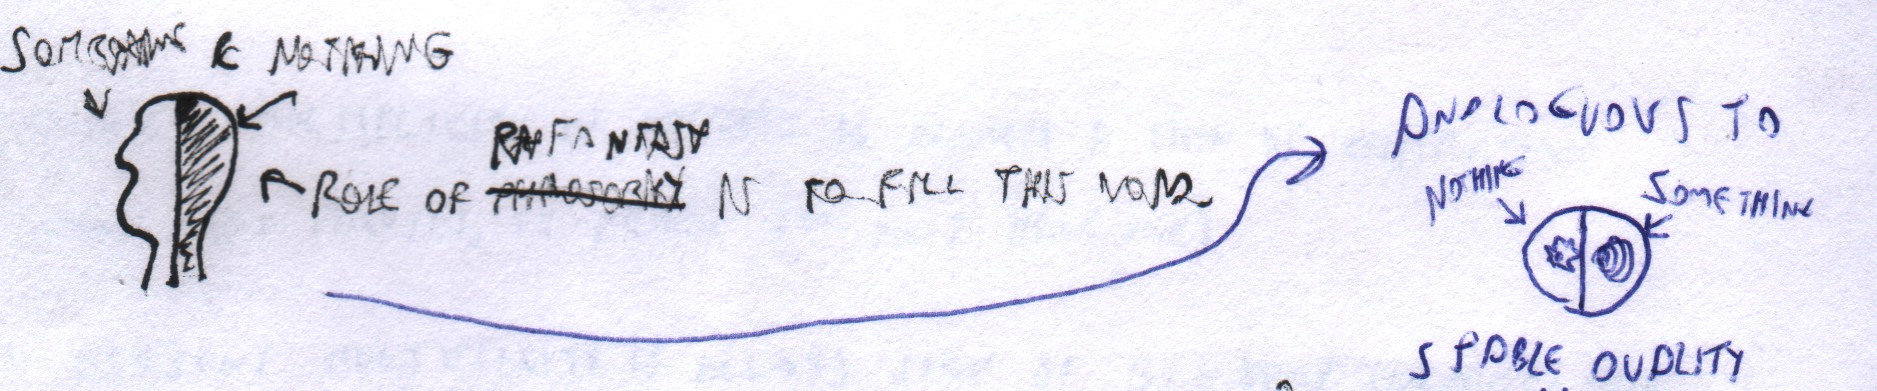
\includegraphics[width=90mm]{scan14.jpg}
%\caption{A simple caption}
\label{overflow}
\end{figure}
 something/nothing -> Role of fantasy is to fill this void.
-We constantly divide subject in two (symmetrically opposite) parts, while at the last division we get subject and nothing (other).
---
Answers:
-Troika: Not "Being qua being as generic multiplicity"
-For Badiou "one" comes secondary. One is an operation, one is an effect of counting, while multiplicity is there from the beginning (multiplicity and void and all that)
-For Alenka and Zizek, there is no original multiplicity, and this absence is inscribed into multiplicity from very beginning (multiplicity is multiplicity without one) -> The one as absence is already here. (One as failed, as impossible)
-Alenka: There is multiplicity because one can not be one.
-Freud (small remark): Multiplicity in dreams is always a sign of castration (if you dream many faluses, it means you don't have one) -> Zizek: Present multiplicity is always sign of blocked/sabotaged one.
-We are tempted to insist on this primacy of the cut/barbed one, of the impossible one. That the one is as it were ..(there us (troika) get really Hegelian).. that there are ones of course, but the existing ones are a echo of their own impossibility (as it were). In a certain way Alain is right: What is, is always originally multiplicity, but why do we then start to count to one? Precisely by the lack or impossibility of the one.
-Badiou: There is multiplicity in logics of the world, and then, I don't know from where all of a sudden there are worlds. I know he would probably reject this as a question, but what I am always asking him is: Why does "Being qua being" (this prerepresentable multiplicity), why does it organize itself into worlds? -Worlds are in a way worlds which appear. Worlds are modes of transcendental appearance.. -Alenka solution: Already multiplicity from the very beginning is the multiplicity, because one is impossible. That this is the answer why multiplicity precisely to fill in this gap, has to appear (to itself).
-For Hegel true enigma is: (not Kantian: We live in appearances, can we reach the thing in itself (the real)) Ok, there is being, multiplicity out there, but why does being start to appear to itself?
-Badiou (too much of the dialectical materialist) vs Zizek (transcendentalist) true fight: Apropo world, the status of the world. Zizek: All the coordinates are already the coordinates of subjective, of universe of (naively) "symbolic universe with subjectivity included" -> there is no world outside language and subject. Badiou insists that world is just a category of what (Engels?) would have called dialectics in nature. If you look at nature: animals, rocks, group of stars; all this can be a world. -> Zizek doubts if this is a legitimate move.
-For Lacan existence (transcendental determination) is absolutely not the same as being. -> In Hegel existence is being which is appearance of some essence. -> For existence you already have to have an essence. 
	*For Lacan neither subject, neither woman exist. (Not to say that there are no woman!) -> There is no big other (He doesn't only say that the big other doesn't exist!) 
	*What doesn't exist insist? (Drive doesn't exist, but the very definition of a drive is that it insists.) -> Subject dosent exist, it just leaves traces in existence.
-Distinction between (in strict lacanian terms) appearance and phenomenon: Appearance being appearance of something, and phenomenon being appearance of nothing. -> (Just raises desire for something behind, but there is nothing behind) appearance is the abyss.
-Lacan: Big other only exists insofar as we believe that it exists. -> Later Lacan: There is no big other. It's non functional even as non existing.
\end{quotation}
======================

\begin{figure}[ht!]
\centering
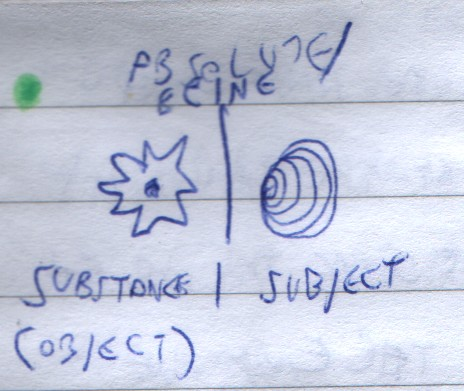
\includegraphics[width=90mm]{scan09.jpg}
%\caption{A simple caption}
\label{overflow}
\end{figure}
[substance (object) +  subject = absolute]
-Linguistics at its purest: Recursion: see recursion.
-So jump and end are only divides (lines) and object and subject are true entities [and other half true? and object a half true?] 
\begin{figure}[ht!]
\centering
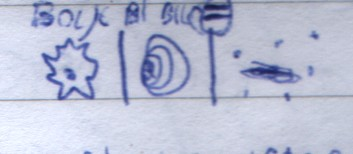
\includegraphics[width=90mm]{scan10.jpg}
%\caption{A simple caption}
\label{overflow}
\end{figure}
So Jump is a harder divide (or maybe just needs a little delay to come to being). So true duality is one between object and subject+other, but other seizes to exist, so we can say object/subject.

-Hegel already in in conclusion of a chapter on consciousness developed something.

-Of course we don't look at the process as having a temporal dimension. So as we speak of primordial singularity, the end (absolute knowledge) already happened, but still we must introduce the notion of a delay. (primordial?) 

%========================================================
%========================================================
%CHAPTER 5
\chapter{A Quick Look at the History}

We could look at the western history as a process whit two camel backs. 
\begin{figure}[ht!]
\centering
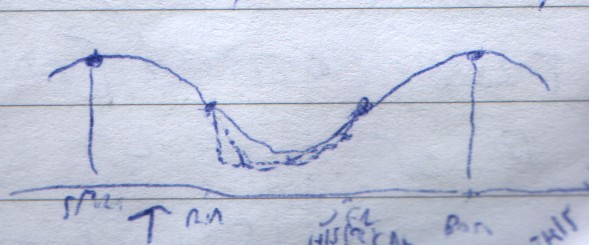
\includegraphics[width=90mm]{scan11.jpg}
%\caption{A simple caption}
\label{overflow}
\end{figure}
So we have death of a Sofocles, fall of Rome, fall of Jerusalem and fall of Bastille/Paris. So the two hills are representing Hellenistic philosophy and German idealism, and the walley the early middle ages.
So, although its hard to deny a sort of fetishism of this approach, it's probably undeniable that Westerners always looked at themselves trough that kind of historical narrative glasses, and  thus, if for nothing else, this already makes the the approach real in a way.

[Todo: aligning my conclusions with a history of philosophy]

\begin{figure}[ht!]
\centering
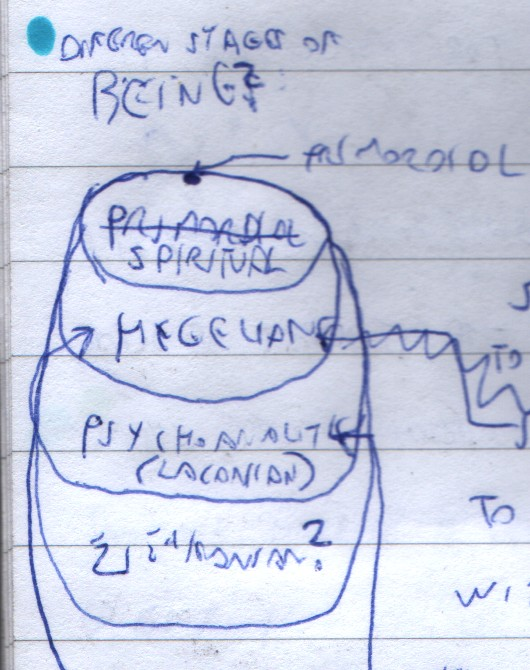
\includegraphics[width=90mm]{scan13.jpg}
%\caption{A simple caption}
\label{overflow}
\end{figure}
Primordial (madness), spiritual, Hegelian (why does it ends/why does it start), lacanian (why do we perceive singularity as being absolute?), zizekanian. 
Different stages of being?

So as showed before, our position in the world (east/west) can probably define us. But there are other things that were with us from the beginning. For instance 5 fingers, and also 5 (non reproductive) limbs. Head + 2 arms + 2 legs (same but mirror images)
So our universe, if we look just to the minimum is what was symbolically saturated from the beginning: 4+1 limbs, 4+1 fingers, 4 ways of a sky + our (central) position ... (4 elements + man) ... Besides those of course there is also duality: woman/man, two parts of a body (l/r)...

%========================================================
%========================================================
%CHAPTER 6
\chapter{List of a Significent Places}

So...

\end{document}
